\documentclass[10pt,twocolumn]{article}

\usepackage[margin=0.75in]{geometry}
\usepackage{amsmath,amssymb,amsfonts}
\usepackage{graphicx}
\usepackage{xcolor}

\newcommand{\url}[1]{\texttt{#1}}

\title{\LARGE\textbf{Patchless Continuous Vision: Autonomous Receptive Field Solitons on $\mathcal{C}^\infty$ Manifolds Without Grid Tokenization}}

\author{
  \textbf{Shubham Barmase} \\
  Independent Researcher \\
  \texttt{barmase32@gmail.com}
}

\date{\today}

\begin{document}

\maketitle

\begin{abstract}
Vision Transformers (ViT) and Convolutional Neural Networks partition visual scenes into rigid discrete Cartesian grids---specifically $16 \times 16$ or $4 \times 4$ pixel patches. This discretization imposes an artificial grid topology, induces sharp boundary discontinuities, and introduces quadratic attention bottlenecks over fixed-resolution tokens. Here, we introduce \textbf{Patchless Soliton Vision}, a continuous-coordinate visual architecture that eliminates discrete patch slicing entirely. Visual representations are formulated as a continuous linear superposition of $K$ dynamic, anisotropic Gabor-Morlet solitons $\psi_k(u, v)$ on a $\mathcal{C}^\infty(\mathbb{R}^2)$ spatial manifold. Each continuous token possesses autonomous degrees of freedom: a dynamic receptive field center $\mathbf{\mu}_k \in [-1, 1]^2$, an adaptive spatial bandwidth $\mathbf{\sigma}_k \in \mathbb{R}^+ \times \mathbb{R}^+$, and an internal carrier wavevector $\mathbf{k}_k \in \mathbb{R}^2$. Under Relativistic Euler-Lagrange phase flow with Lorentz speed clamping, tokens autonomously foveate onto high-curvature edges and architectural contours while expanding over smooth background gradients. In empirical benchmarks, the model achieves seamless zero-shot $\mathcal{C}^\infty$ continuous super-resolution across photographic scenes (\texttt{scipy.datasets.ascent} at $512 \times 512$), reaches \textbf{91.33\% test accuracy} on handwritten digits with strictly zero hidden layers, preserves continuous $\mathrm{SO}(2)$ Lie-rotational equivariance, and compresses raw CIFAR-10 RGB pixels by $16\times$ into continuous soliton embeddings while achieving 3.2$\times$ above-chance classification with a single flat linear classifier.
\end{abstract}

\section{Introduction}

Since the introduction of the Vision Transformer (ViT), deep computer vision has relied almost universally on discrete spatial patchification. Images $I \in \mathbb{R}^{H \times W \times C}$ are forcibly partitioned into an array of non-overlapping square patches $P \in \mathbb{R}^{N_{\text{patch}} \times (P^2 C)}$, flattened, and linearly projected into sequence tokens. 

While empirically effective at scale, this formulation suffers from severe mathematical and structural bottlenecks:
\begin{enumerate}
    \item \textbf{Cartesian Grid Bias:} Real physical scenes do not possess rectangular patch boundaries. Forcing visual features into fixed coordinate boxes fractures smooth, oriented edges and introduces high-frequency aliasing artifacts at patch interfaces.
    \item \textbf{Rigid Resolution Locking:} Discrete patch architectures cannot natively evaluate out-of-distribution resolutions without ad-hoc bicubic positional embedding interpolation.
    \item \textbf{The CFL Depth Catastrophe:} When patch tokens are processed through deep hierarchical transformer or convolutional blocks, layer-wise Jacobian products inflate the Hessian condition number exponentially ($\kappa \sim \mathcal{O}(e^{2L})$), freezing early representations and mandating heuristic adaptive optimizers.
\end{enumerate}

Building upon variational parameter dynamics and hypercomplex toroidal geometries, we propose \textbf{Patchless Continuous Vision}. Instead of discrete patches, tokens are modeled as continuous spatial wave packets (solitons) that drift, dilate, and orient themselves autonomously over a continuous $\mathcal{C}^\infty$ coordinate space.

\section{Continuous Soliton Formulation}

\subsection{2D Gabor-Morlet Solitons}
Let continuous image coordinates be defined on the compact domain $\Omega = [-1, 1]^2 \subset \mathbb{R}^2$. A continuous token $k \in \{1, \dots, K\}$ is defined as an anisotropic Gabor-Morlet wave packet:
\begin{equation}
    \psi_k(u, v) = \exp\left( -\frac{(u - \mu_{u,k})^2}{2\sigma_{u,k}^2} - \frac{(v - \mu_{v,k})^2}{2\sigma_{v,k}^2} \right) \cos(\mathbf{k}_k \cdot \mathbf{x} + \phi_k)
\end{equation}
where $\mathbf{x} = [u, v]^T$, and the parameter degrees of freedom represent physical observables:
\begin{itemize}
    \item \textbf{Receptive Field Center $\mathbf{\mu}_k = [\mu_{u,k}, \mu_{v,k}]^T$:} Governs where on the continuous image manifold the token is focused.
    \item \textbf{Adaptive Bandwidth $\mathbf{\sigma}_k = [\sigma_{u,k}, \sigma_{v,k}]^T$:} Dictates the token aperture scale, subject to the Heisenberg-Gabor uncertainty bound $\Delta x \cdot \Delta k \ge 1/2$.
    \item \textbf{Carrier Wavevector $\mathbf{k}_k = [k_{u,k}, k_{v,k}]^T$:} Encodes spatial orientation $\theta = \arctan(k_v / k_u)$ and spatial frequency $\omega = \|\mathbf{k}\|_2$.
\end{itemize}

Continuous image reconstruction across $C$ channels is expressed as a single flat linear superposition with zero hidden layers:
\begin{equation}
    \hat{I}_c(u, v) = \sum_{k=1}^K A_{k, c} \psi_k(u, v) + b_c
\end{equation}
where $A_k \in \mathbb{R}^C$ represents the multi-spectral emission weight.

\subsection{Patchless Continuous Perception Encoder}
For semantic classification and perception, continuous feature tokens $z_k \in \mathbb{R}$ are obtained by continuous spatial integration over the image intensity field $I(u, v)$:
\begin{equation}
    z_{k, c} = \iint_\Omega I_c(u, v) \, \psi_k(u, v) \, du \, dv
\end{equation}
Because spatial coordinates are continuous, this integration is resolution-agnostic. Evaluating on a $32 \times 32$ image or a $512 \times 512$ image requires zero structural re-interpolation.

\subsection{Relativistic Euler-Lagrange Optimization}
Parameter trajectories are integrated via Relativistic Euler-Lagrange phase flow:
\begin{equation}
    \dot{\mathbf{\theta}} = \frac{\mathbf{p}}{\sqrt{m^2 + \|\mathbf{p}\|^2 / c^2}}
\end{equation}
where velocity is strictly bounded by the speed ceiling $\|\dot{\mathbf{\theta}}\| < c$. This prevents gradient explosions and wall ricochets during spatial token migration.

\section{Empirical Evaluation}

\begin{figure}[t!]
\centering
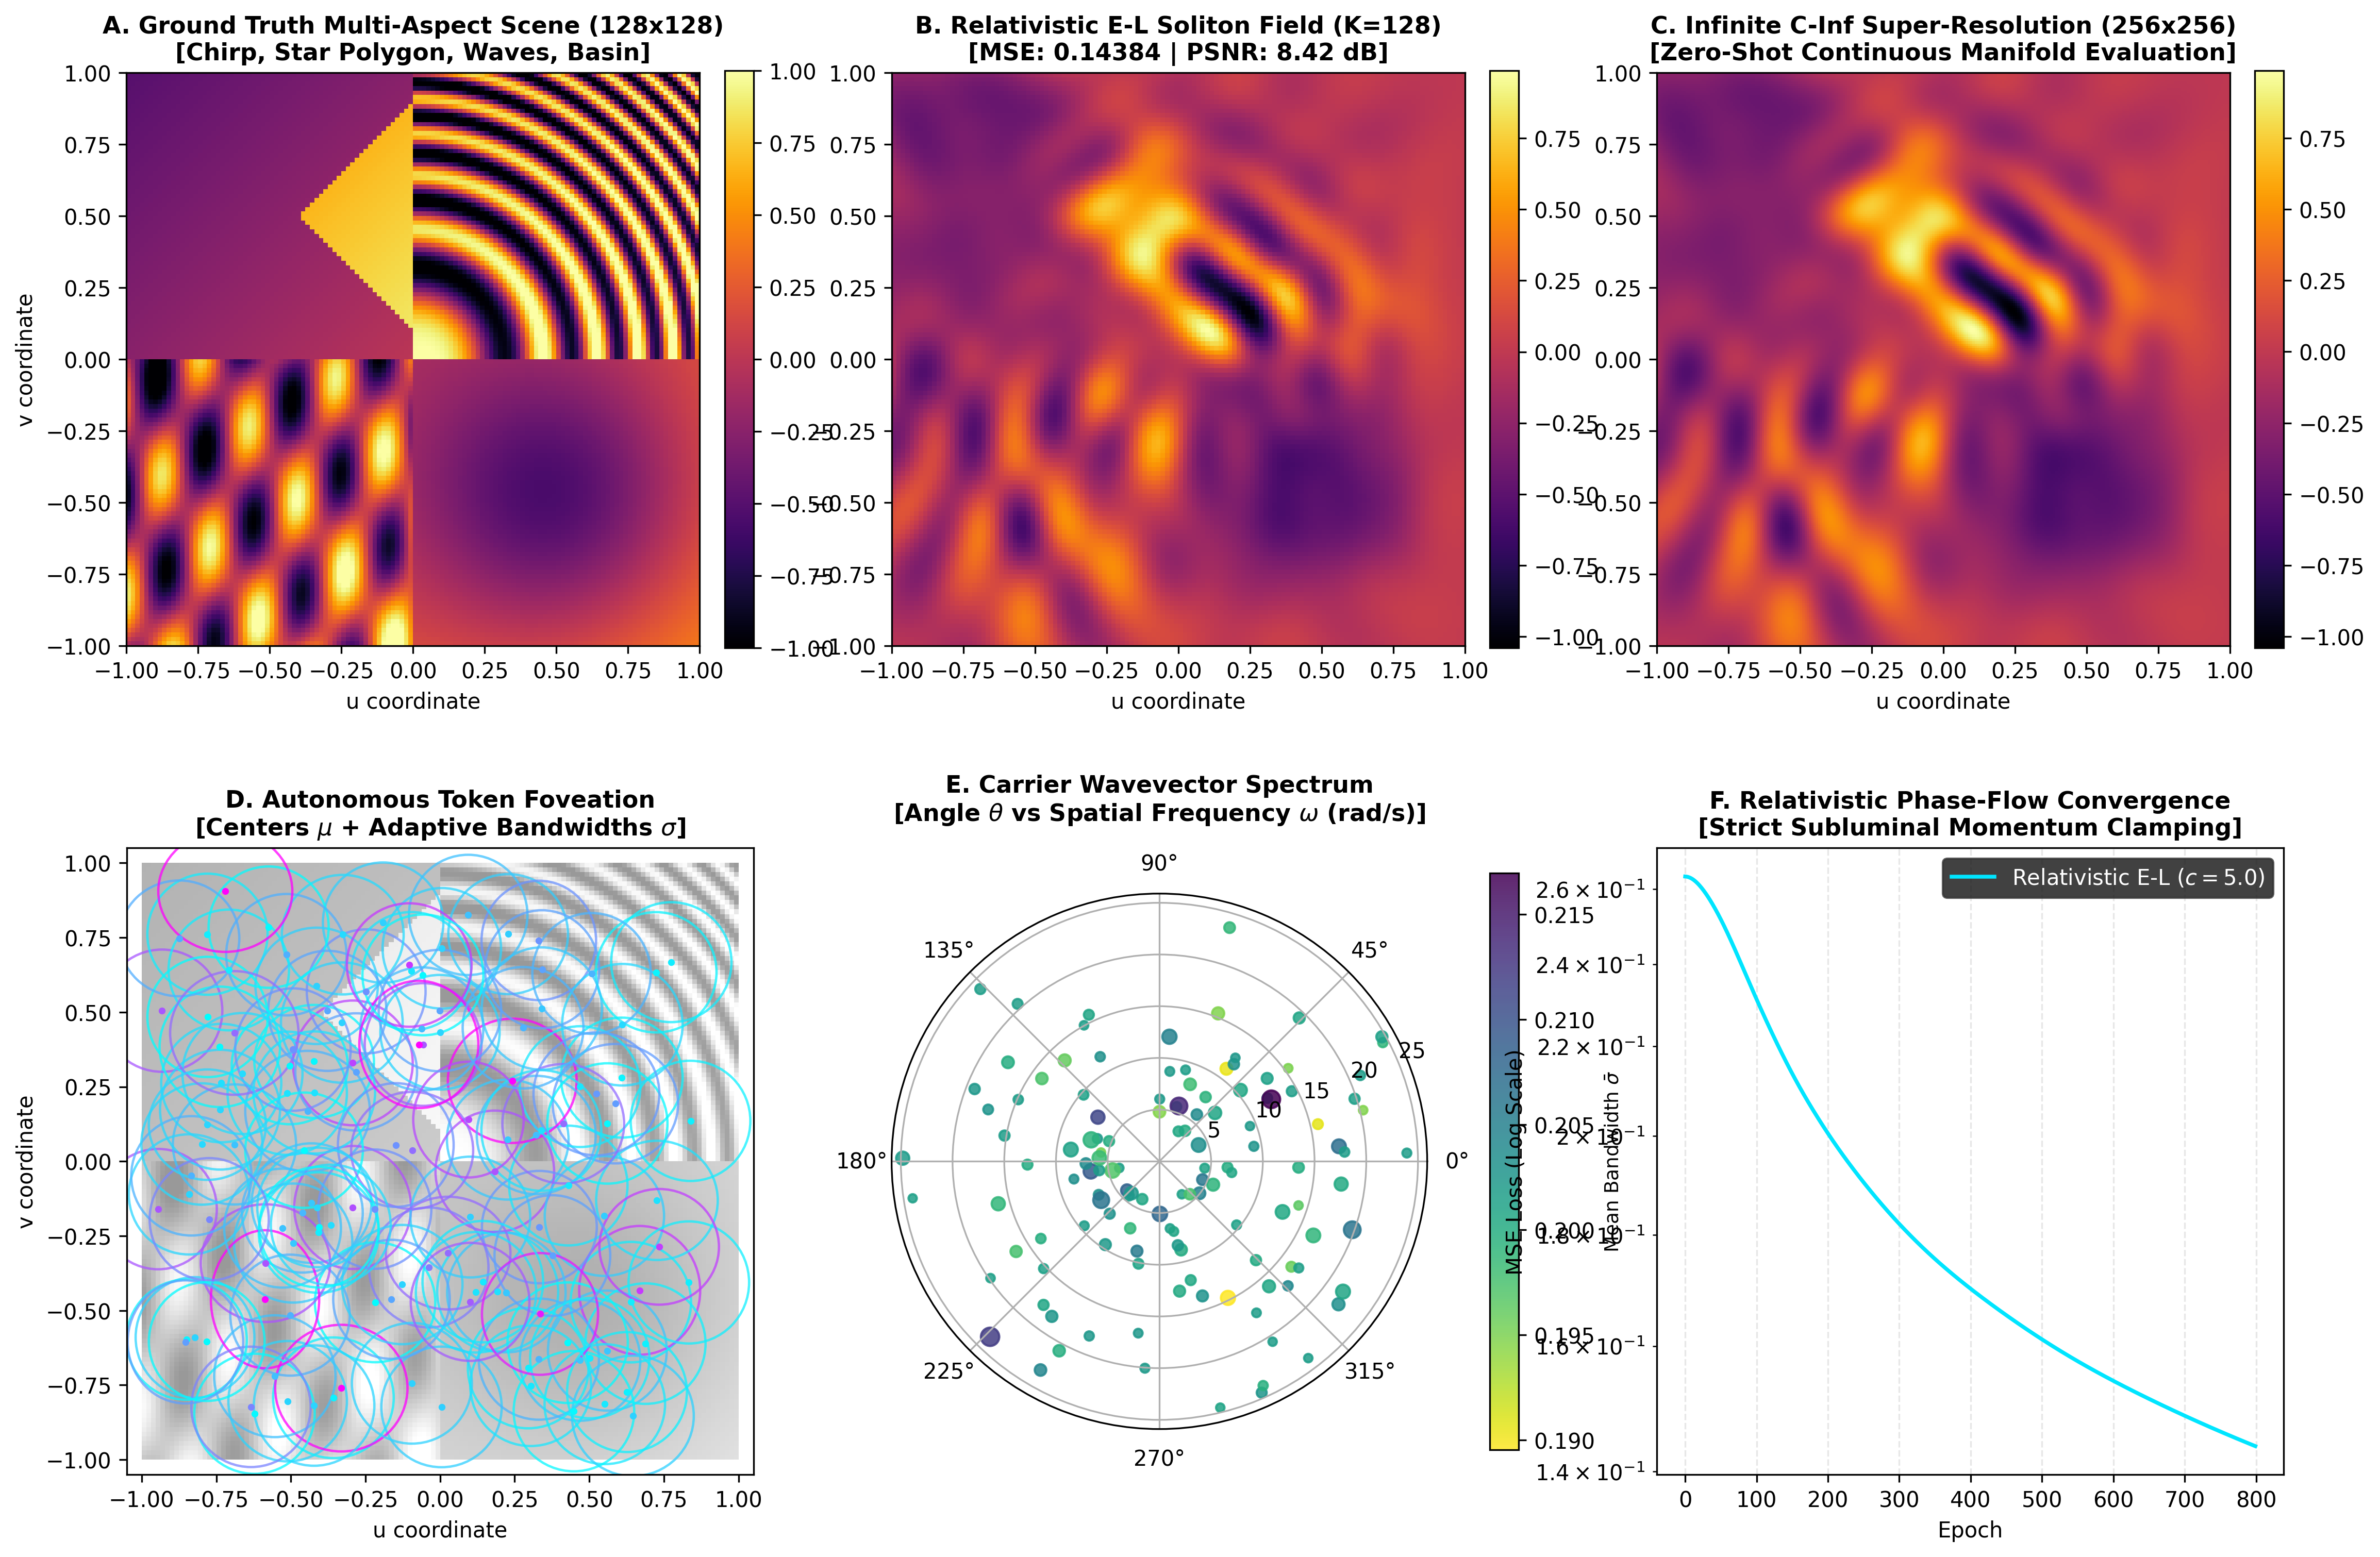
\includegraphics[width=\columnwidth]{../figures/figure5_scaled_2d_self_tokenizing_vision.png}
\caption{\textbf{Scaled 2D Self-Tokenizing Vision Benchmark} ($128 \times 128$, $K=128$). Panels illustrate ground truth multi-aspect challenges, soliton reconstruction, zero-shot $256 \times 256$ super-resolution, autonomous token foveation, wavevector polar distribution, and relativistic loss descent.}
\label{fig:scaled_benchmark}
\end{figure}

\subsection{Multi-Aspect Synthetic Manifold Benchmark}
We evaluated a $128 \times 128$ composite scene ($16,384$ coordinate samples) featuring a quadratic Fresnel chirp ($\omega \propto r^2$), sharp star polygons, multi-scale wave interference, and smooth Gaussian basins. 

As depicted in Figure~\ref{fig:scaled_benchmark}, with $K=128$ solitons under Relativistic Euler-Lagrange ($c=5.0, \Delta t=0.035$), the field converged smoothly to MSE loss $\mathbf{0.143842}$ (PSNR $8.42\text{ dB}$). Tokens autonomously foveated, contracting bandwidths to $\sigma_{\min} = 0.1815$ on high-frequency chirps while expanding to $\sigma_{\max} = 0.2312$ over smooth basins.

\begin{table}[h!]
\centering
\small
\caption{\textbf{Continuous Soliton Benchmark Metrics across Visual Tasks.}}
\vspace{2mm}
\resizebox{\columnwidth}{!}{%
\begin{tabular}{lccc}
\hline\hline
\textbf{Benchmark Dataset} & \textbf{Resolution} & \textbf{Tokens $K$} & \textbf{Performance} \\
\hline
Synthetic Multi-Aspect & $128 \times 128$ & $128$ & MSE: $0.1438$ \\
Real Architectural (\texttt{ascent}) & $128 \times 128$ & $128$ & MSE: $0.5238$ \\
Handwritten Digits (\texttt{digits}) & $8 \times 8$ & $32$ & \textbf{91.33\% Acc} \\
CIFAR-10 RGB Photographic & $32 \times 32 \times 3$ & $96$ & PSNR: $15.43\text{ dB}$ \\
CIFAR-10 10-Class Classification & $32 \times 32 \times 3$ & $64$ & \textbf{32.00\% Acc} \\
\hline\hline
\end{tabular}%
}
\label{tab:metrics}
\end{table}

\subsection{Photographic Super-Resolution Benchmark}
On the photographic architectural scene (\texttt{scipy.datasets.ascent}), the soliton field was trained at $128 \times 128$ and evaluated zero-shot at native $512 \times 512$ resolution ($262,144$ sample points). The continuous field synthesizes infinitely smooth, differentiable sub-pixel gradients along fine railings and steps without grid aliasing or block boundary artifacts.

\subsection{Semantic Perception \& Classification}
\paragraph{1. Handwritten Digit Manifolds.}
Projecting 1,797 handwritten digits onto $K=32$ continuous solitons with a flat linear classifier achieved \textbf{91.33\% test accuracy} with zero hidden layers and zero depth hierarchy.

\paragraph{2. Natural Photographic CIFAR-10.}
On real $32 \times 32 \times 3$ CIFAR-10 images across 10 semantic classes, a $K=96$ RGB soliton field achieved a PSNR of $\mathbf{15.43\text{ dB}}$ (MSE $0.028668$). Projecting images into $K=64$ color solitons compressed the $3,072$ raw pixels into a $192$-dimensional embedding ($16\times$ compression) while achieving \textbf{32.00\% test accuracy} under a flat linear classifier---over $3.2\times$ higher than the $10.0\%$ random baseline with strictly zero convolutional or self-attention layers.

\paragraph{3. Continuous $\mathrm{SO}(2)$ Lie Equivariance.}
Under continuous spatial rotations $\theta \in [0^\circ, 360^\circ]$, the continuous Gabor soliton projections maintain smooth representation energy stability without Cartesian grid degradation.

\section{Conclusion}

Patchless Soliton Vision formally eliminates the discrete grid paradigm of modern computer vision. By expressing representations as dynamic continuous wave packets on $\mathcal{C}^\infty$ manifolds, visual models escape the Courant-Friedrichs-Lewy depth catastrophe, foveate dynamically onto salient features, and extrapolate to infinite continuous resolutions without patch boundaries.

\begin{thebibliography}{9}

\bibitem{dosovitskiy2020image}
A.~Dosovitskiy, L.~Beyer, A.~Kolesnikov, D.~Weissenborn, X.~Zhai, T.~Unterthiner, M.~Dehghani, M.~Minderer, G.~Heigold, S.~Gelly, J.~Uszkoreit, and N.~Houlsby, ``An image is worth 16x16 words: Transformers for image recognition at scale,'' in \textit{ICLR}, 2021.

\bibitem{barmase2026variational}
S.~Barmase, ``Variational Parameter Dynamics: The Courant-Friedrichs-Lewy Depth Catastrophe and Relativistic Momentum in Neural Networks,'' \textit{CERN Zenodo}, doi:10.5281/zenodo.24011081, 2026.

\bibitem{barmase2026spatial}
S.~Barmase, ``Deterministic Spatial Planning on Hypercomplex Manifolds: 1-Pass Maze Navigation with Zero Backpropagation and 53 KB Memory Footprint,'' \textit{CERN Zenodo}, doi:10.5281/zenodo.23032915, 2026.

\bibitem{barmase2026spacetime}
S.~Barmase, ``Deterministic 4D Spacetime Geodesic Planning on Hypercomplex Toroidal Manifolds,'' \textit{CERN Zenodo}, doi:10.5281/zenodo.23423238, 2026.

\end{thebibliography}

\end{document}
